% !TEX root = meca1321-synthesis.tex

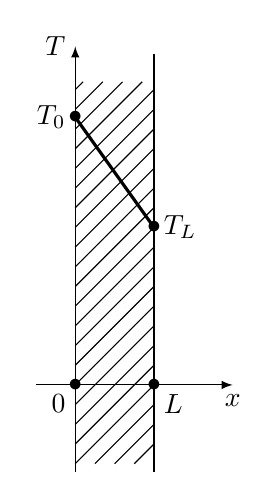
\begin{tikzpicture}
  \draw [>=latex, ->] (-0.5, 0) -- (2, 0);
  \draw [>=latex, ->] (0, -1.1) -- (0, 4.3);
  \draw (0, 0) node {$\bullet$};
  \draw (0, 0) node [below left] {$0$};
  \draw (1, 0) node {$\bullet$};
  \draw (1, 0) node [below right] {$L$};
  \draw (1, -1.1) -- (1, 4.2);
  \draw (0, 4.3) node [left] {$T$};
  \draw (2, 0) node [below] {$x$};
  \foreach \i in {-4, ..., 11}
  {
    \pgfmathsetmacro{\x}{(\i/4)};
    \draw (0, \x) -- ++(1, 1);
  }
  \draw (0.25, -1) -- ++(0.75, 0.75);
  \draw (0.50, -1) -- ++(0.5, 0.5);
  \draw (0.75, -1) -- ++(0.25, 0.25);
  \draw (0, 3) -- ++(0.85, 0.85);
  \draw (0, 3.25) -- ++(0.6, 0.6);
  \draw (0, 3.5) -- ++(0.35, 0.35);
  \draw (0, 3.75) -- ++(0.1, 0.1);
  \draw (0, 3.4) node {$\bullet$};
  \draw (1, 2.0) node {$\bullet$};
  \draw [line width = 0.4mm] (1, 2.0) -- (0, 3.4);
  \draw (0, 3.4) node [left] {$T_0$};
  \draw (1, 2.0) node [right] {$T_L$};
\end{tikzpicture}
